\begin{figure*}[t]
  \centering
  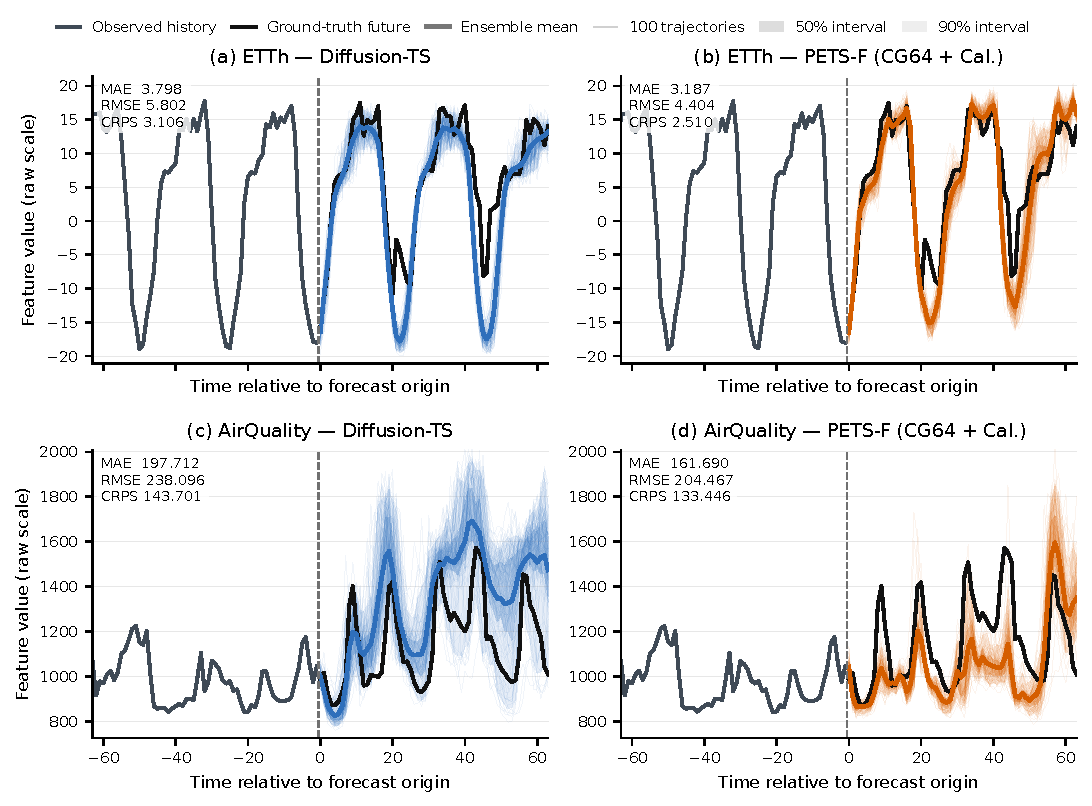
\includegraphics[width=\textwidth]{figs/probabilistic_forecasting_main_v3.pdf}
  \caption{Qualitative probabilistic forecasts on illustrative FINAL_TEST windows where the final PETS-F configuration yields lower ensemble-mean MAE and empirical CRPS than Diffusion-TS under a fixed seed-0 selection ensemble. To avoid extreme or best-case examples, candidate windows are restricted to the central 20--80\% of ground-truth curvature, variability, amplitude range, and boundary-jump statistics, and the case closest to the median joint PETS improvement is shown. Thin curves denote 100 stochastic trajectories, the thick forecast curve their pointwise ensemble mean, and the shaded bands the 50\% and 90\% central prediction intervals. The quantitative FINAL_TEST comparison over all windows and three model seeds is reported separately in Table X.}
  \label{fig:probabilistic-forecasting-qualitative-v3}
\end{figure*}
